\documentclass[17pt]{beamer}
  \usepackage[czech]{babel}
  \usepackage[utf8]{inputenc}
  \usepackage[T1]{fontenc}
  \usepackage{textcomp}
  \usepackage{color}

  \usetheme{Boadilla}
  \usecolortheme{beaver}

  \title[Kalendář]{Elektronický kalendář}
  \subtitle{Projekt do ITU, 2013}
  \author[Zadání 23]{Michal Duban \and Marko Fábry \and Jan Wrona}
  \institute[FIT VUT]{Vysoké učení technické v Brně}

\begin{document}
\frame{\titlepage}

\begin{frame}{Výsledná aplikace}
\begin{itemize}
    \item vykreslení kalendáře na pracovní plochu
    \item zobrazení pro týden a měsíc
    \item zvýraznění aktuálního dne
    \item čísla týdnů
\end{itemize}
\end{frame}

\begin{frame}{Zaměření projektu}
\begin{itemize}
    \item zobrazení a editace kalendářových dat
    \item praktičnost
    \item žádné rušivé elementy
\end{itemize}
\end{frame}

\begin{frame}{Hypotéza / Idea}
\begin{itemize}
    \item dnešní řešení: google calendar, rainlendar, samurize
    \item naše řešení: na ploše je kalendář často na očích
    \item cílová skupina: lidé, kteří potřebují mít přehled o plánovaných aktivitách
    \item verze řešení: obrázek, okno
\end{itemize}
\end{frame}

\begin{frame}{Detaily návrhu}
\begin{itemize}
    \item obrázek: menší variabilita
    \item specifika implementace: multiplatformnost, změna pozice
\end{itemize}
\end{frame}

\begin{frame}{Realizace}
\begin{itemize}
    \item implementace v C++, Qt, QML
    \item click-through, průhlednost
    \item multiplatformnost: makra, WinAPI
\end{itemize}
\end{frame}

\begin{frame}{Měsíc}
    \begin{center}
    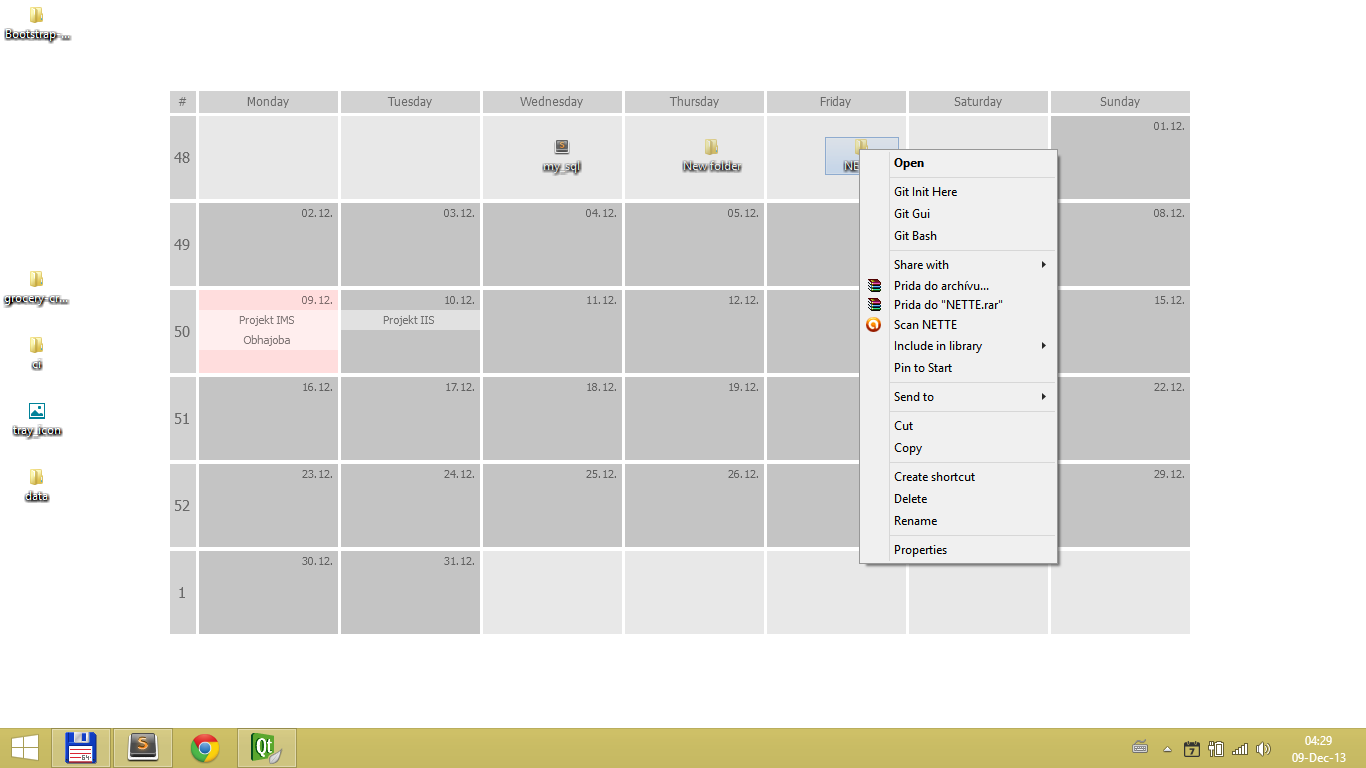
\includegraphics[width=\textwidth,height=\textheight,keepaspectratio]{monthscreen.png}
    \end{center}
\end{frame}

\begin{frame}{Tray menu}
    \begin{center}
    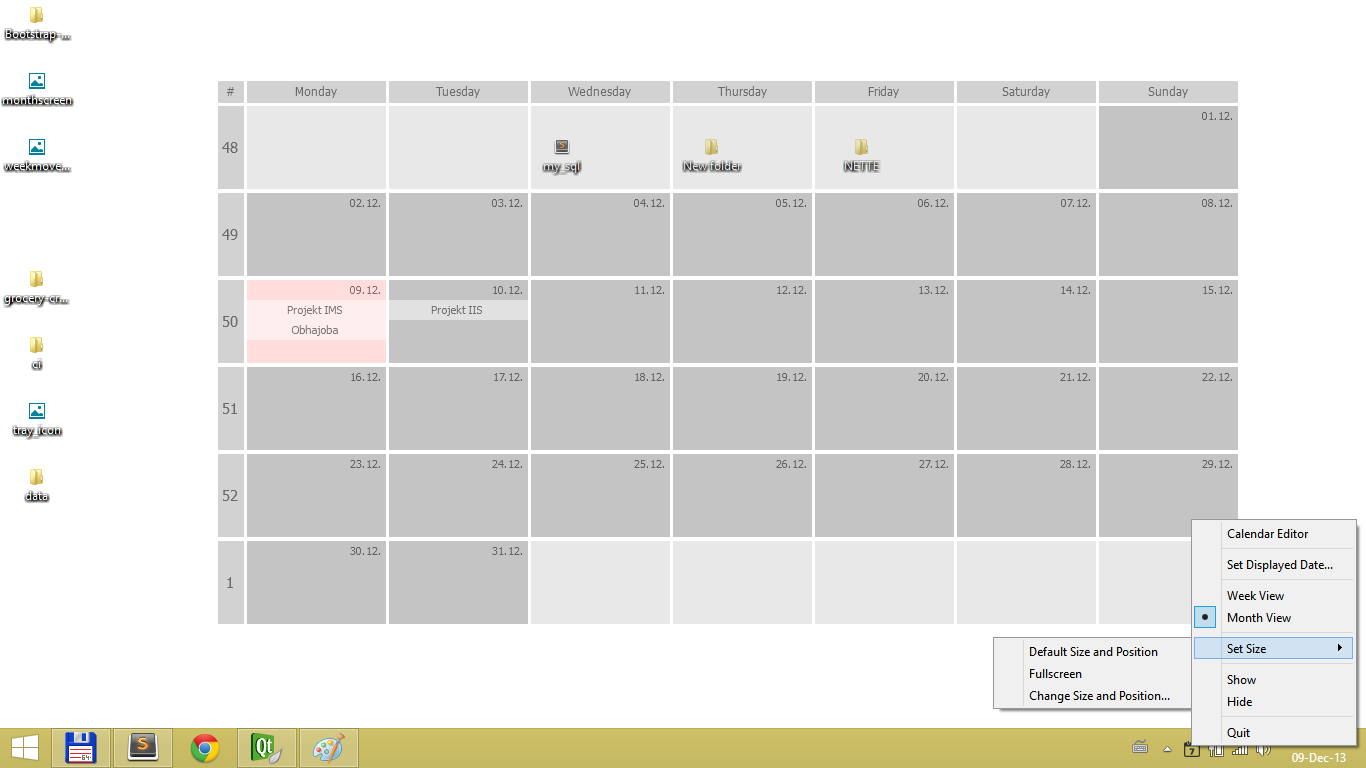
\includegraphics[width=\textwidth,height=\textheight,keepaspectratio]{weekmovescreen.png}
    \end{center}
\end{frame}

\begin{frame}{Google login}
    \begin{center}
    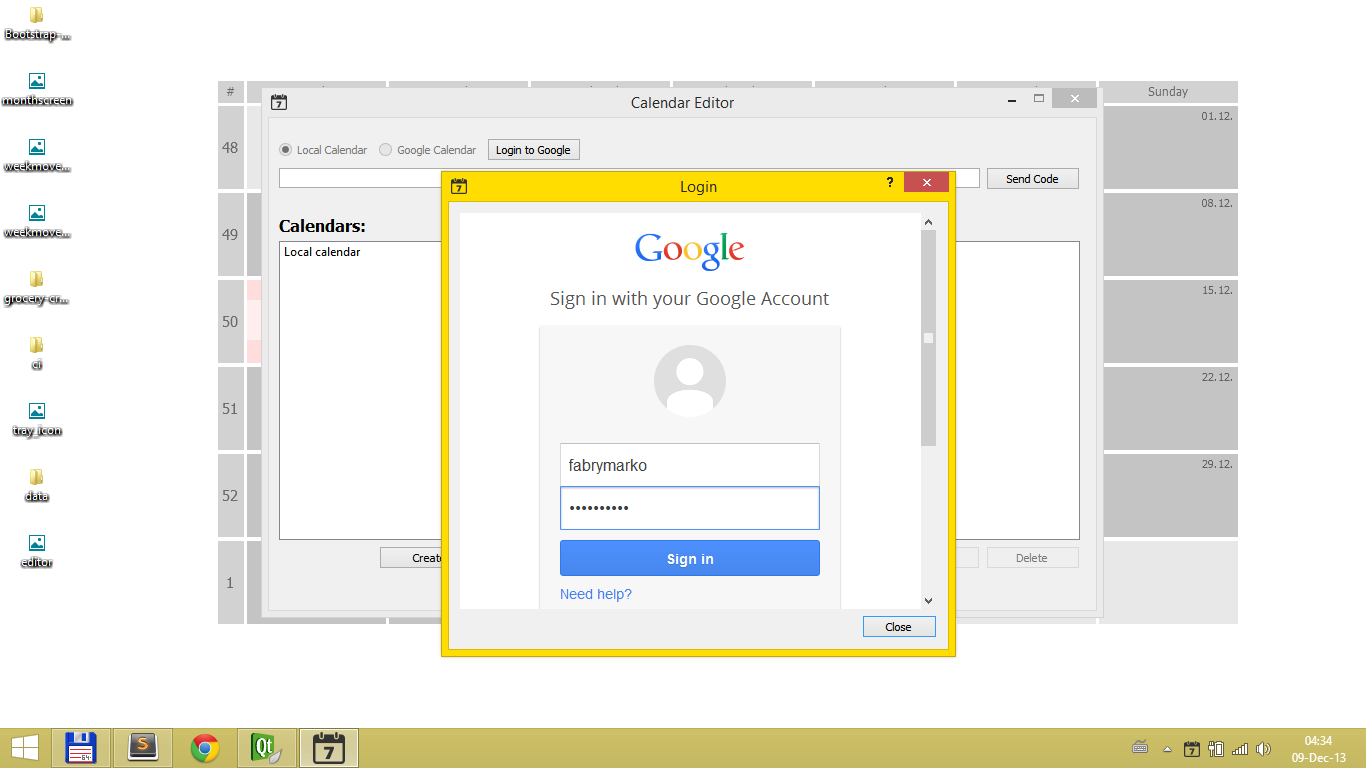
\includegraphics[width=\textwidth,height=\textheight,keepaspectratio]{googlelogin.png}
    \end{center}
\end{frame}

\begin{frame}{Editor kalendářů}
    \begin{center}
    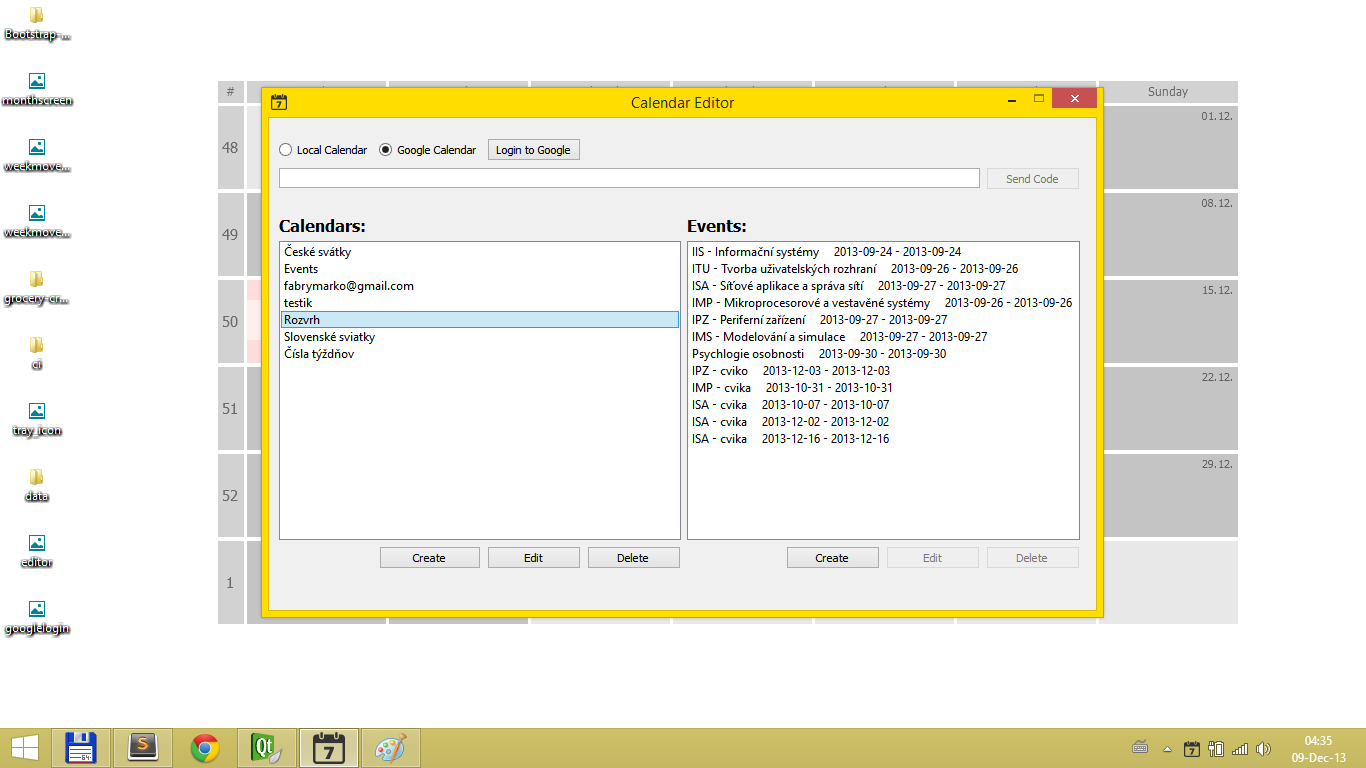
\includegraphics[width=\textwidth,height=\textheight,keepaspectratio]{editorgoogle.png}
    \end{center}
\end{frame}

\begin{frame}{Testování}
\begin{itemize}
    \item 2x měření doby stejných úkolů
    \item důvody: 1. intuitivnost 2. přehlednost
    \item 9 lidí, neinformatici, naši vrstevníci
    \item ne vždy stejná vývojový verze
\end{itemize}
\end{frame}

\begin{frame}{Testování}
\begin{table}[h]
{\tiny
    \begin{center}
    \begin{tabular}{| c | c | c | c || c | c | c |}
    \hline
     & \multicolumn{3}{|c||}{Pokus č. 1} & \multicolumn{3}{c|}{Pokus č. 2}\\
    Uživatel & a & b & c & a & b & c \\
    \hline
    Hana D. & 69 & 9 & 17 & 34 & 4 & 10 \\
    Martin D. & 32 & 5 & 11 & 28 & 3 & 7 \\
    Martin P. & 53 & 10& 19 & 31 & 7 & 6 \\
    Michal K. & 71 & 5 & 12 & 38 & 4 & 7 \\
    Tomáš P. & 66 & 7 & 18 & 40 & 5 & 8 \\
    Vít M. & 60 & 7 & 12 & 25 & 6 & 9 \\
    Gabina J. & 51 & 9 & 17 & 34 & 8 & 6 \\
    Petr C. & 71 & 8 & 17 & 37 & 4 & 10 \\
    Bianka F. & 74 & 8 & 16 & 29 & 6 & 14 \\
    \hline
    Průměr: & 60.77 & 7.55 & 15.44 & 32.88 & 5.22 & 8.55\\
    \hline
    \end{tabular}
    \caption{Tabulka výsledků}
    \label{tab:vysledky}
    \end{center}
   }
\end{table}
\end{frame}

\begin{frame}{Výsledky}
\begin{itemize}
    \item rozdíl mezi prvním a "rutinním" použitím
    \item aplikace je nenápadná
    \item snadná orientace a rychlá akce
\end{itemize}
\end{frame}

\begin{frame}{Na co jsme z řešení nejvíce hrdí?}
\begin{itemize}
    \item implementace
\end{itemize}
\end{frame}

\begin{frame}
\begin{center}
    {\LARGE Děkujeme za pozornost.}
\end{center}
\end{frame}

\end{document}
